\section{Balanced Clustering}
\label{sec:imbalance}

Task clustering has been widely used to address the low performance of very short running tasks on platforms where the system overhead is high, such as distributed computing infrastructures. However, up to now, techniques do not consider the load balance problem. In particular, merging tasks within a workflow level without considering the runtime variance may cause load imbalance (Runtime Imbalance), or merging tasks without considering their data dependencies may lead to data locality problems (Dependency Imbalance). In this section, we introduce metrics that quantitatively capture workflow characteristics to measure runtime and dependence imbalances. We then present methods to handle the load balance problem.

\begin{figure}[!t]
\centering
 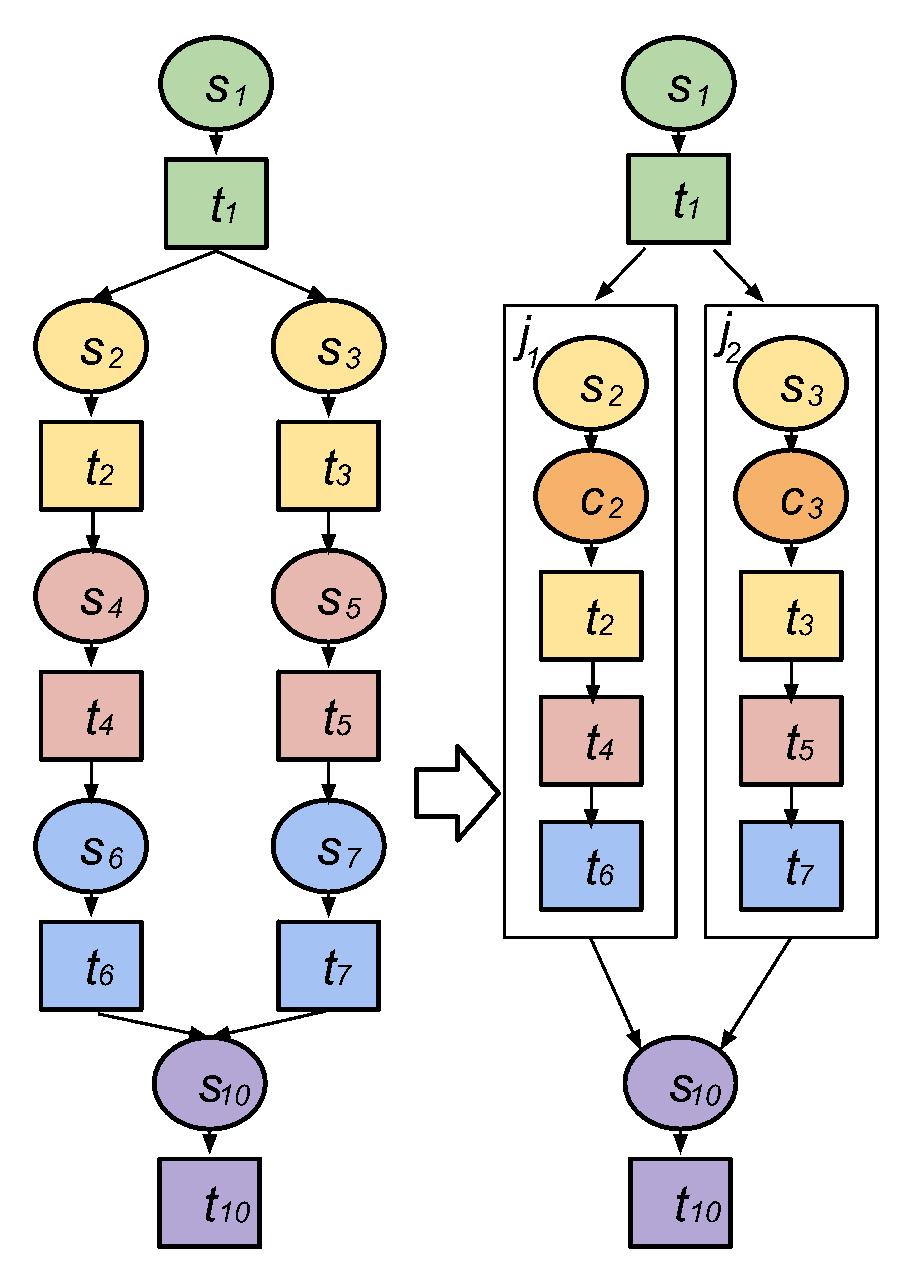
\includegraphics[width=0.55\linewidth]{figure4.eps}
  \captionof{figure}{An example of vertical clustering.}
  \label{fig:model_vc}
\end{figure}

\subsection{Imbalance metrics}

\textbf{Runtime Imbalance} describes the difference of the task/job runtime of a group of tasks/jobs. In this work, we denote the \textbf{Horizontal Runtime Variance} ($HRV$) as the ratio of the standard deviation in task runtime to the average runtime of tasks/jobs at the same horizontal level of a workflow. At the same horizontal level, the job with the longest runtime often controls the release of the next level jobs. A high $HRV$ value means that the release of next level jobs has been delayed. Therefore, to improve runtime performance, it makes sense to reduce the standard deviation of job runtime. Figure~\ref{fig:imbalance_rv} shows an example of four independent tasks $t_1$, $t_2$, $t_3$ and $t_4$ where the task runtime of $t_1$ and $t_2$ is 10 seconds, and the task runtime of $t_3$ and $t_4$ is 30 seconds. In the Horizontal Clustering (HC) approach, a possible clustering result could be \rev{to merge }$t_1$ and $t_2$ into a clustered job, and $t_3$ and $t_4$ into another. This approach results in imbalanced runtime, i.e., $HRV > 0$ (Figure~\ref{fig:imbalance_rv}-top). In contrast, a balanced clustering strategy should try its best to evenly distribute task runtime among jobs as shown in Figure~\ref{fig:imbalance_rv} (bottom). A smaller \emph{HRV} means that the runtime of tasks within a horizontal level is more evenly distributed and therefore it is less necessary to use runtime-based balancing algorithms. However, runtime variance is not able to \rev{capture }how symmetric the structure of the dependencies between tasks is.

\begin{figure}[htb]
	\centering
	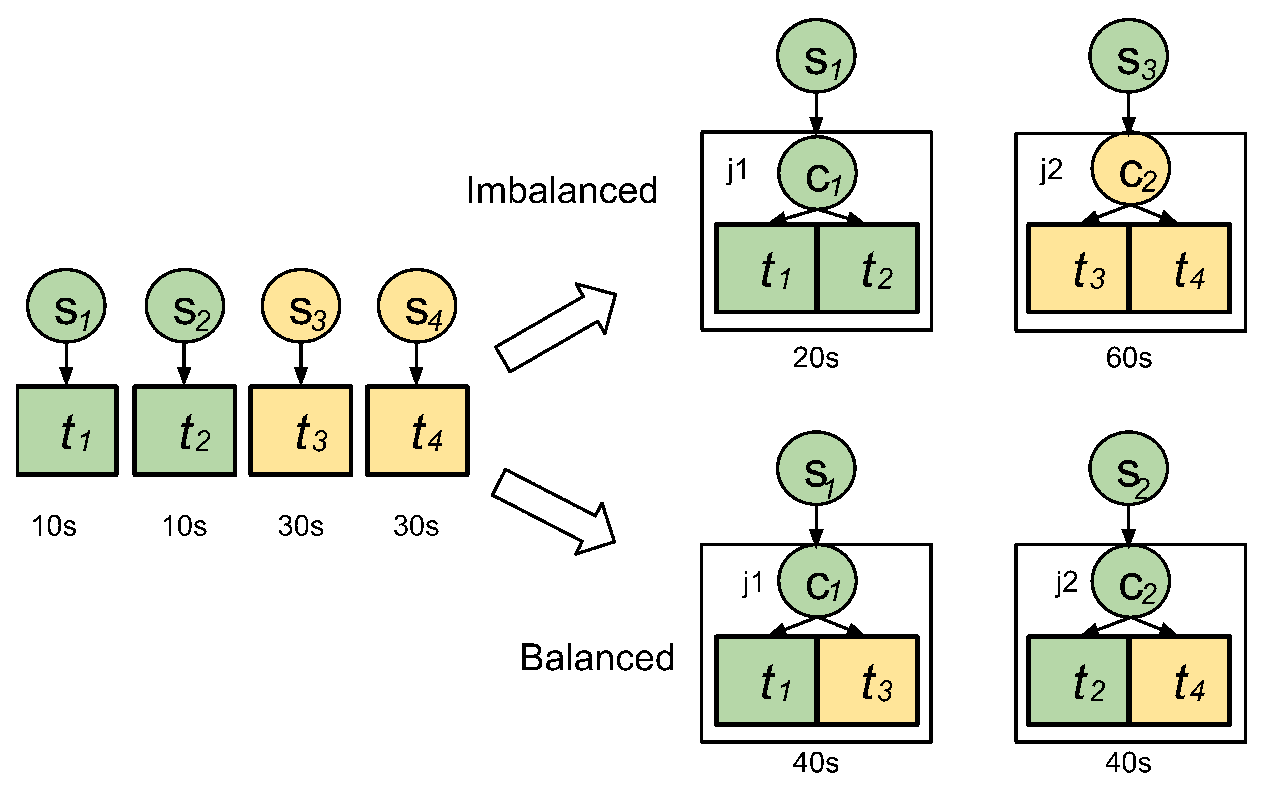
\includegraphics[width=0.95\linewidth]{figure5.eps}
	\captionof{figure}{An example of Horizontal Runtime Variance.}
	\label{fig:imbalance_rv}
\end{figure}


\textbf{Dependency Imbalance} means that the task clustering at one horizontal level forces the tasks at the next level (or even subsequent levels) to have severe data locality problems and thus loss of parallelism. For example, in Figure~\ref{fig:imbalance_dv}, we show a two-level workflow composed of four tasks in the first level and two in the second. Merging $t_1$ with $t_3$ and $t_2$ with $t_4$ (imbalanced workflow in Figure~\ref{fig:imbalance_dv}) forces $t_5$ and $t_6$ to transfer files from two locations and wait for the completion of $t_1$, $t_2$, $t_3$, and $t_4$.  A balanced clustering strategy groups tasks that have the maximum number of child tasks in common. Thus, $t_5$ can start to execute as soon as $t_1$ and $t_2$ are completed, and so can $t_6$. To \rev{quantitatively measure }the Dependency Imbalance of a workflow, we propose two  metrics: ($i$) Impact Factor Variance, and ($ii$) Distance Variance. 

\begin{figure}[htb]
	\centering
	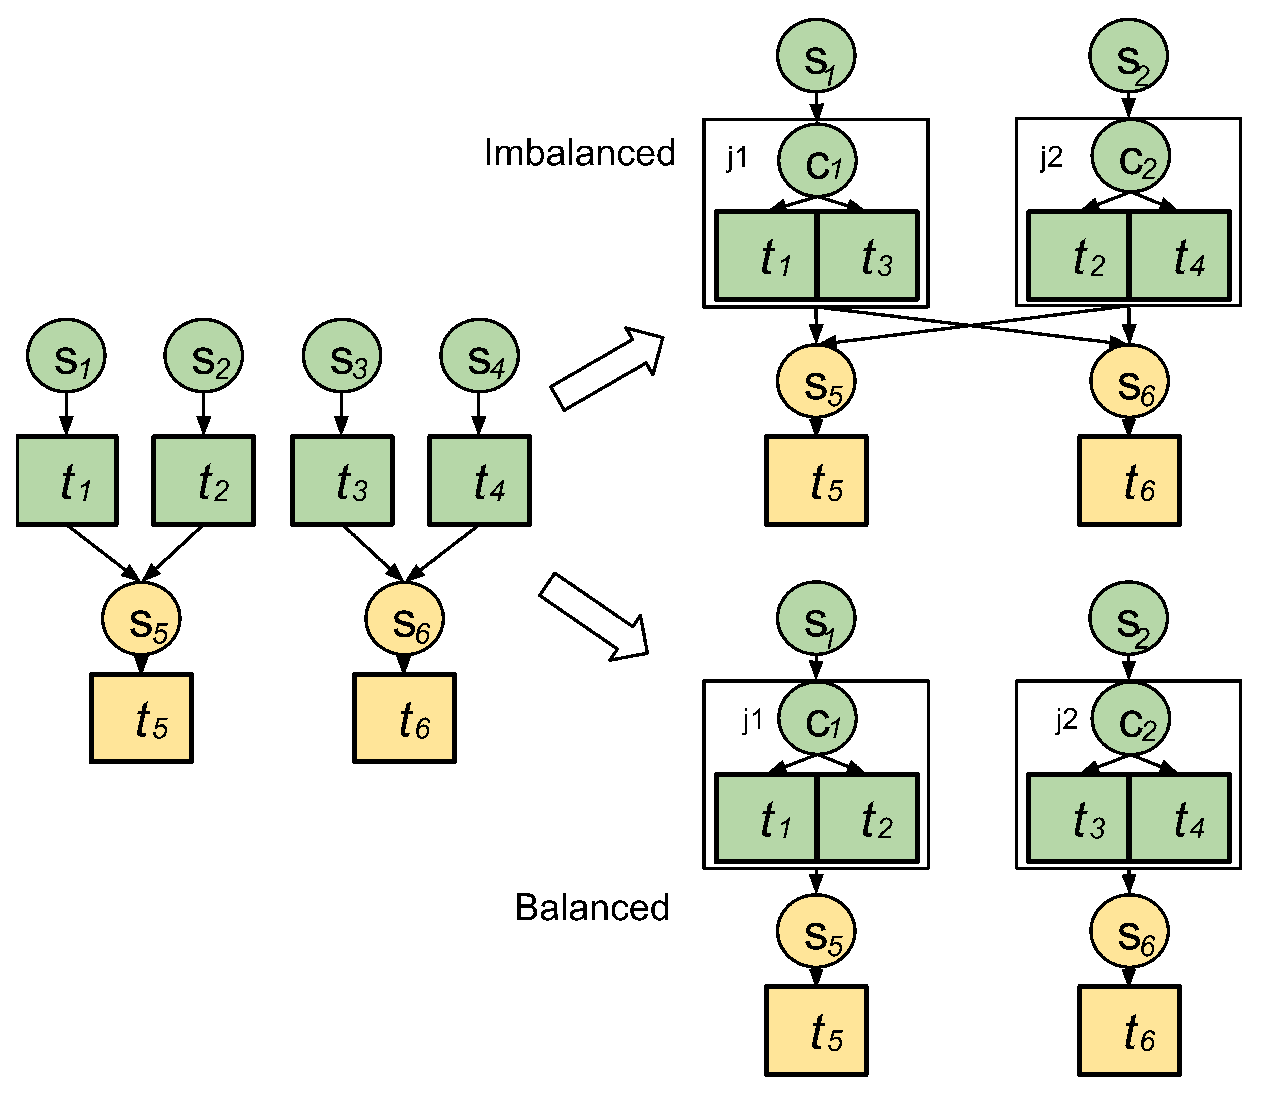
\includegraphics[width=0.95\linewidth]{figure6.eps}
	\captionof{figure}{An example of Dependency Imbalance.}
	\label{fig:imbalance_dv}
\end{figure}

We define the \textbf{Impact Factor Variance} ($IFV$) of tasks as the standard deviation of their impact factors. The \textbf{Impact Factor} ($IF$) of a task $t_u$ is defined as follows:

\begin{equation}
\label{eq:imbalance_impact_factor}
	IF(t_u)=\sum_{t_v\in Child(t_u)}^{}\frac{IF(t_v)}{||Parent(t_v)||}
\end{equation}
where $Child(t_u)$ denotes the set of child tasks of $t_u$, and $||Parent(t_v)||$ the number of parent tasks of $t_v$. The Impact Factor aims \rev{to capture }the similarity of tasks/jobs in a graph by measuring their relative impact factor or importance to the entire graph. Tasks with similar impact factors are merged together, so that the workflow structure tends to be more \rev{``even'' }or symmetric. For simplicity, we assume the $IF$ of a workflow exit task (\rev{a task without children}, e.g. $t_5$ in Figure~\ref{fig:imbalance_dv}) is 1.0. \rev{Consider }the two workflows presented in Figure~\ref{fig:imbalance_hifv}. The $IF$ for each of $t_1$, $t_2$, $t_3$, and $t_4$ is computed as follows:
\begin{eqnarray}
	\displaystyle  
	&IF(t_7 )=1.0, IF(t_6 )=IF(t_5 )=IF(t_7 )/2=0.5\nonumber  \\
	&IF(t_1 )=IF(t_2 )=IF(t_5 )/2=0.25\nonumber \\
	&IF(t_3 )=IF(t_4 )=IF(t_6 )/2=0.25\nonumber 
\end{eqnarray}
Thus, IFV($t_1$, $t_2$, $t_3$, $t_4$) = 0. In contrast, the $IF$ for $t_{1'}$, $t_{2'}$, $t_{3'}$, and $t_{4'}$ is:
\begin{eqnarray}
	\displaystyle  
	&IF(t_{7'})=1.0, IF(t_{6'})=IF(t_{5'})=IF(t_{1'})=IF(t_{7'})/2=0.5\nonumber \\
	&IF(t_{2'})=IF(t_{3'})=IF(t_{4'})=IF(t_{6'})/3=0.17 \nonumber
\end{eqnarray}
Therefore, the $IFV$ value for {$t_{1'}$, $t_{2'}$, $t_{3'}$, $t_{4'}$} is 0.17, which predicts \rev{that }it is likely to be less symmetric than the workflow in Figure~\ref{fig:imbalance_hifv} (left). In this paper, we use \textbf{HIFV} (Horizontal IFV) to indicate the $IFV$ of tasks at the same horizontal level. The time complexity of calculating the $IF$ of all the tasks of a workflow with $n$ tasks is $O(n)$.  

\begin{figure}[htb]
	\centering
	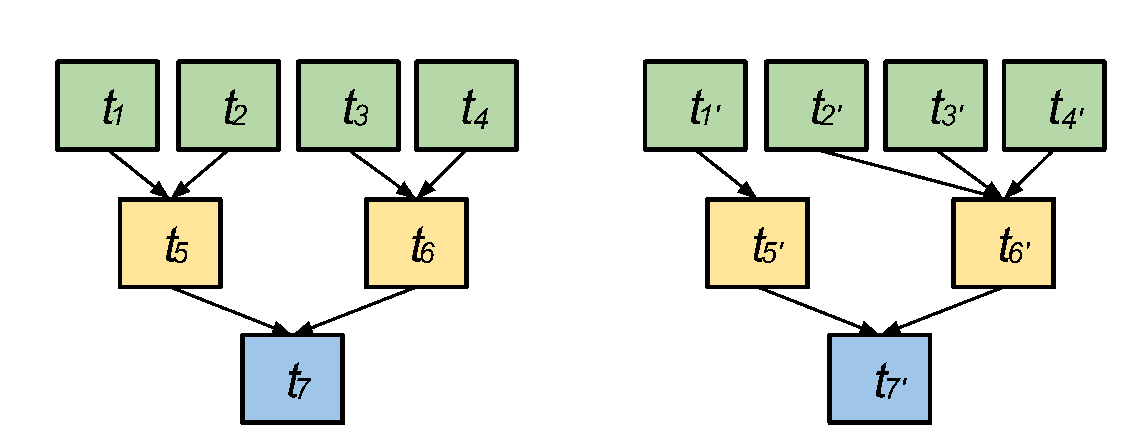
\includegraphics[width=0.85\linewidth]{figure7.eps}
	\captionof{figure}{Example of workflows with different data dependencies (For better visualization, we do not show system overheads in the rest of the paper).}
	\label{fig:imbalance_hifv}
\end{figure}

\textbf{Distance Variance} ($DV$) describes how `close' tasks are to each other. The distance between two tasks/jobs is defined as the \rev{sum of the distance to }their closest common successor. If they do not have a common successor, the distance is set to infinity. For a group of $n$ tasks/jobs, the distance between them is represented by a $n \times n$ matrix $D$, where an element $D(u,v)$ denotes the distance between a pair of tasks/jobs $u$ and $v$. For any workflow structure, $D(u,v)=D(v,u)$ and $D(u,u)=0$, thus we ignore the cases when $u \geq v$. Distance Variance is then defined as the standard deviation of all the elements $D(u,v)$ for $u<v$. The time complexity of calculating all the values of $D$ of a workflow with $n$ tasks is $O(n^2)$. 

Similarly, $HDV$ indicates the $DV$ of a group of tasks/jobs at the same horizontal level. For example, Table~\ref{tab:imblance_metric} shows the distance matrices of tasks from the first level for both workflows of Figure~\ref{fig:imbalance_hifv} ($D_1$ for the workflow in the left, and $D_2$ for the workflow in the right). $HDV$ for $t_1, t_2, t_3$, and $t_4$ is 1.03, and for $t_{1'}, t_{2'}, t_{3'}$, and $t_{4'}$ is 1.10. In terms of distance variance, $D_1$ is more \rev{``even'' }than $D_2$. A smaller $HDV$ means the tasks at the same horizontal level are more equally \rev{``distant'' }from each other and thus the workflow structure tends to be more \rev{``even'' }and symmetric. 

\begin{table}[htb]
	\footnotesize
	\centering
	\begin{tabular}{l|rrrr}
		$D_1$ & $t_1$ & $t_2$ & $t_3$ &$t_4$\\
		\hline
		$t_1$ & 0 & 2 & 4 & 4 \\
		$t_2$ & 2 & 0 & 4 & 4 \\
		$t_3$ & 4 & 4 & 0 & 2\\
		$t_4$ & 4 & 4 & 2 & 0 \\
	\end{tabular}
	\quad
	\begin{tabular}{l|rrrr}
		$D_2$ & $t_1'$ & $t_2'$ & $t_3'$ &$t_4'$\\
		\hline
		$t_1'$ & 0 & 4 & 4 & 4 \\
		$t_2'$ & 4 & 0 & 2 & 2 \\
		$t_3'$ & 4 & 2 & 0 & 2\\
		$t_4'$ & 4 & 2 & 2 & 0 \\
	\end{tabular}
	\caption{Distance matrices of tasks from the first level of workflows in Figure~\ref{fig:imbalance_hifv}.}
	\label{tab:imblance_metric}
\end{table}

In conclusion, runtime variance and dependency variance offer a quantitative and comparable tool to measure and evaluate the internal structure of a workflow. 



\subsection{Balanced clustering methods}
\label{sec:methods}
In this subsection, we introduce our balanced clustering methods used to improve the runtime and dependency balances in task clustering. We first \rev{present }the basic runtime-based clustering method, and then two other balancing methods that address the dependency imbalance problem. %We use the metrics presented in the previous subsection to evaluate a given workflow to decide which balancing method(s) is(are) more appropriate. 

%Algorithm~\ref{alg:imbalance_algo} shows the pseudocode of our balanced clustering algorithm that uses a combination of these balancing methods and metrics.  The maximum number of clustered jobs (size of $CL$) is equal to the number of available resources multiplied by a \emph{clustering factor}. 

%\begin{algorithm}[htb]
%	\caption{ Balanced Clustering algorithm}
%	\footnotesize
%	\label{alg:imbalance_algo}
%	\begin{algorithmic}[1]
%		\Require $W$: workflow; $CL$: list of clustered jobs; $C$: the required size of $CL$; 
%		\Ensure The job runtime of $CL$ are as even as possible
%		\Procedure{Clustering}{$W,D,C$}
%			\State Sort $W$ in decreasing order of the size of each level
%			\For{$level < $the depth of $W$}
%				\State $TL\gets $\ \Call{GetTasksAtLevel}{$w,level$} \Comment{Partition $W$ based on depth}
%				\State $CL\gets$  \ \Call{Merge}{$TL,C$} \Comment{Form a list of clustered jobs}
%				\State $W \gets W - TL + CL$  \Comment{Merge dependencies as well} 
%			\EndFor
%		\EndProcedure
%		\Procedure{Merge}{$TL, C$}
%			\State Sort $TL$ in decreasing order of task runtime
%			\For{$t\ in\ TL$}
%				\State $J \gets $\ \Call{GetCandidateJob}{$CL, t$} \Comment{Get a candidate task}
%				\State  $J \gets J\ +\ t$ \Comment{Merge it with the clustered job}
%			\EndFor
%			\State \textbf{return} $CL$
%		\EndProcedure
%		\Procedure{GetCandidateJob}{$CL, t$}
%			\State Selects a job based on balanced clustering methods
%		\EndProcedure
%	\end{algorithmic}
%\end{algorithm}

%We examine tasks in a level-by-level approach starting from the level with the largest width (number of tasks at the same level, \texttt{line 2}). The intuition behind this breadth favored approach is that we believe it should improve the performance most. Then, we determine which type of imbalance problem a workflow experiences based on the balanced clustering metrics presented previously ($HRV$, $HIFV$, and $HDV$), and accordingly, we select a combination of balancing methods. \textsc{GetCandidateJob} selects a job (\texttt{line 12}) from a list of potential candidate jobs ($CL$) to be merged with the targeting task ($t$). Below we introduce the three balancing methods proposed in this work.


\begin{algorithm}[!htb]
	\footnotesize
	\caption{Horizontal Runtime Balancing algorithm.}
	\label{alg:imbalance_hrb}
	\begin{algorithmic}[1]
		\Require $W$: workflow; $R$: number of jobs per horizontal level
		\Procedure{Clustering}{$W,R$}
			\For{$level < depth(W)$}
				\State $TL\gets $\ \Call{GetTasksAtLevel}{$W,level$} \Comment{Partition $W$ based on depth}
				\State $C \gets TL.size() / R$ \Comment{$C$ is number of tasks per job in this level}
				\State $CL\gets$  \ \Call{Merge}{$TL,C, R$} \Comment{Returns a list of clustered jobs}
				\State $W \gets W - TL + CL$  \Comment{Merge dependencies as well} 
			\EndFor
		\EndProcedure
		\Procedure{Merge}{$TL, C, R$}
			\For{$i<R$}
			\State $J_i\gets$\{\}\Comment{An empty job}
			\EndFor
			\State $CL\gets$\{\}\Comment{An empty list of clustered jobs}
			\State Sort $TL$ in descending of runtime
			\ForAll{$t$ in $TL$}
				\State $J\gets$ the job with shortest runtime and less than $C$ tasks  
				\State $J$.add ($t$) \Comment{Adds the task to the shortest job}
				
			\EndFor
			\For{$i<R$}
			\State  $CL$.add( $J_i$)
			\EndFor
			\State \textbf{return} $CL$
		\EndProcedure
	\end{algorithmic}
\end{algorithm}



\textbf{Horizontal Runtime Balancing} (HRB) aims to evenly distribute task runtime among clustered jobs. Tasks with the longest runtime are added to the job with the shortest runtime. Algorithm~\ref{alg:imbalance_hrb} shows the pseudocode of HRB. This greedy method is used to address the load balance problem caused by runtime variance at the same horizontal level. Figure~\ref{fig:imbalance_hrb} shows an example of HRB where tasks in the first level have different runtimes and should be grouped into two jobs. HRB sorts tasks in decreasing order of runtime, and then adds the task with the highest runtime to the group with the shortest aggregated runtime. Thus, $t_1$ and $t_3$, as well as $t_2$ and $t_4$ are merged together.
For simplicity, system overheads are not displayed.

\begin{figure}[htb]
	\centering
	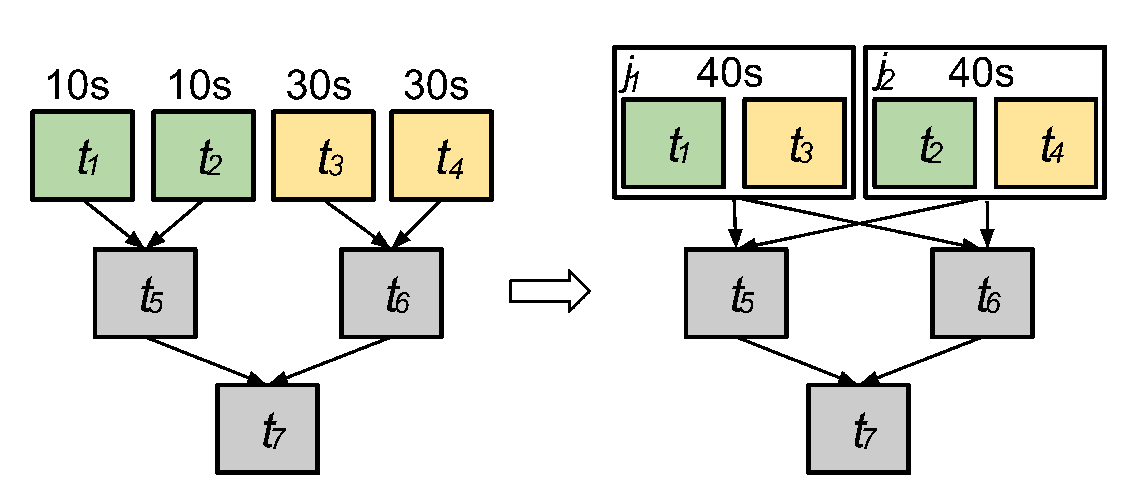
\includegraphics[width=0.85\linewidth]{figure8.eps}
	\caption{An example of the HRB (Horizontal Runtime Balancing) method. By solely addressing runtime variance, data locality problems may arise.}
	\label{fig:imbalance_hrb}
\end{figure}

\begin{algorithm}[!htb]
	\footnotesize
	\caption{Horizontal Impact Factor Balancing algorithm.}
	\label{alg:imbalance_hifb}
	\begin{algorithmic}[1]
		\Require $W$: workflow; $R$: number of jobs per horizontal level
		\Procedure{Clustering}{$W,R$}
			\For{$level < depth(W)$}
				\State $TL\gets $\ \Call{GetTasksAtLevel}{$W,level$} \Comment{Partition $W$ based on depth}
				\State $C \gets TL.size() / R$ \Comment{$C$ is number of tasks per job in this level}
				\State $CL\gets$  \ \Call{Merge}{$TL,C, R$} \Comment{Returns a list of clustered jobs}
				\State $W \gets W - TL + CL$  \Comment{Merge dependencies as well} 
			\EndFor
		\EndProcedure
		\Procedure{Merge}{$TL, C, R$}
			\For{$i<R$}
			\State $J_i\gets$\{\}\Comment{An empty job}
			\EndFor
			\State $CL\gets$\{\}\Comment{An empty list of clustered jobs}
			\State Sort $TL$ in descending of runtime
			\ForAll{$t$ in $TL$}
				\State $L\gets$ Sort all $J_i$ with the similarity of impact factors with $t$
				\State $J\gets$ the job with shortest runtime and less than $C$ tasks in $L$
				\State $J$.add ($t$) 
				
			\EndFor
			\For{$i<R$}
			\State  $CL$.add( $J_i$)
			\EndFor
			\State \textbf{return} $CL$
		\EndProcedure
	\end{algorithmic}
\end{algorithm}


\begin{algorithm}[!htb]
	\footnotesize
	\caption{Horizontal Distance Balancing algorithm.}
	\label{alg:imbalance_hdb}
	\begin{algorithmic}[1]
		\Require $W$: workflow; $R$: number of jobs per horizontal level
		\Procedure{Clustering}{$W,C$}
			\For{$level < depth(W)$}
				\State $TL\gets $\ \Call{GetTasksAtLevel}{$W,level$} \Comment{Partition $W$ based on depth}
				\State $C \gets TL.size() / R$ \Comment{$C$ is number of tasks per job in this level}
				\State $CL\gets$  \ \Call{Merge}{$TL,C, R$} \Comment{Returns a list of clustered jobs}
				\State $W \gets W - TL + CL$  \Comment{Merge dependencies as well} 
			\EndFor
		\EndProcedure
		\Procedure{Merge}{$TL, C, R$}
			\For{$i<R$}
			\State $J_i\gets$\{\}\Comment{An empty job}
			\EndFor
			\State $CL\gets$\{\}\Comment{An empty list of clustered jobs}
			\State Sort $TL$ in descending of runtime
			\ForAll{$t$ in $TL$}
				\State $L\gets$ Sort all $J_i$ with the closest distance with $t$
				\State $J\gets$ the job with shortest runtime and less than $C$ tasks in $L$
				\State $J$.add ($t$) 
				
			\EndFor
			\For{$i<R$}
			\State  $CL$.add( $J_i$)
			\EndFor
			\State \textbf{return} $CL$
		\EndProcedure
	\end{algorithmic}
\end{algorithm}


%how HRB works in an example of four jobs with different job runtime (assuming the height of a job is its runtime). For the given task ($t_0$), HRB sorts the potential jobs ($j_1$, $j_2$, $j_3$, and $j_4$) based on their runtime and selects the shortest job (in this case $j_1$ or $j_2$). 



However, HRB may cause a dependency imbalance problem since the clustering does not take data dependency into consideration. To address this problem, we propose the \textbf{Horizontal Impact Factor Balancing} (HIFB) and the \textbf{Horizontal Distance Balancing} (HDB) methods. 

In HRB, candidate jobs within a workflow level are sorted by their runtime, while in HIFB jobs are first sorted based on their similarity of $IF$, then \rev{based }on runtime. 
Algorithm~\ref{alg:imbalance_hifb} shows the pseudocode of HIFB. 
For example, in Figure~\ref{fig:imbalance_hifb}, $t_1$ and $t_2$ have $IF = 0.25$, while $t_3$, $t_4$, and $t_5$ have $IF = 0.16$. HIFB selects a list of candidate jobs with the same IF value, and then HRB is performed to select the shortest job. Thus, HIFB merges $t_1$ and $t_2$ together, as well as $t_3$ and $t_4$.

\begin{figure}[htb]
	\centering
	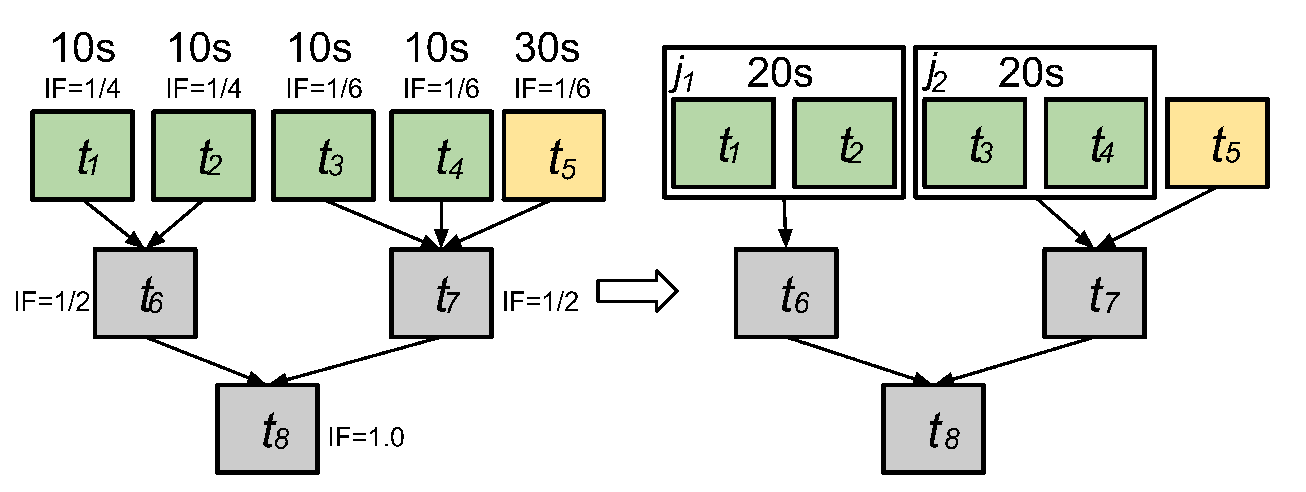
\includegraphics[width=\linewidth]{figure9.eps}
	\captionof{figure}{An example of the HIFB (Horizontal Impact Factor Balancing) method. Impact factors allow the detection of similarities between tasks.}
	\label{fig:imbalance_hifb}
\end{figure}

However, HIFB is \rev{often }suitable for workflows with \rev{an }asymmetric structure. A symmetric workflow structure means there exists a (usually vertical) division of the workflow graph such that one part of the workflow is a mirror of the other part. For symmetric workflows, such as the one shown in Figure~\ref{fig:imbalance_hrb}, the $IF$ value for all tasks of the first level will be the same ($IF=0.25$), thus the method may also cause dependency imbalance. In HDB, jobs are sorted based on the distance between them and the targeted task $t$, then on their runtimes. 
Algorithm~\ref{alg:imbalance_hdb} shows the pseudocode of HDB. 
For instance, in Figure~\ref{fig:imbalance_hdb}, the distances between tasks $D(t_1,t_2)=D(t_3,t_4)=2$, while $D(t_1,t_3)=D(t_1,t_4)=D(t_2,t_3)=D(t_2,t_4)=4$. Thus, HDB merges a list of candidate tasks with the minimal distance ($t_1$ and $t_2$, and $t_3$ and $t_4$). Note that even if the workflow is asymmetric (Figure~\ref{fig:imbalance_hifb}), HDB would obtain the same result as with HIFB. 

\begin{figure}[!htb]
	\centering
	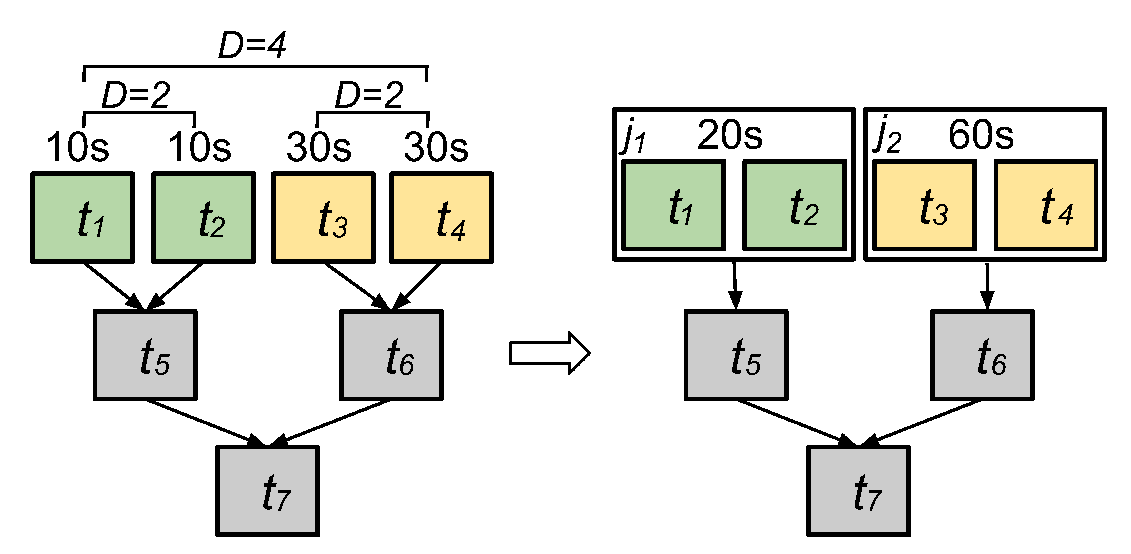
\includegraphics[width=0.85\linewidth]{figure10.eps}
	\captionof{figure}{An example of the HDB (Horizontal Distance Balancing) method. Measuring the distances between tasks avoids data locality problems.}
	\label{fig:imbalance_hdb}
\end{figure}

There are cases where HDB would yield lower performance than HIFB. For instance, let $t_1$, $t_2$, $t_3$, $t_4$, and $t_5$ be the set of tasks to be merged in the workflow presented in Figure~\ref{fig:imbalance_hifb_hdb}. HDB does not identify the difference in the number of parent/child tasks between the tasks, since $d(t_u,t_v) = 2, \forall u,v \in [1,5], u \neq v$. On the other hand, HIFB does distinguish \rev{between } them since their impact factors are slightly different. Example of such scientific workflows include the LIGO Inspiral workflow~\cite{LIGO}, which is used in the evaluation of this paper (Section~\ref{sec:results}).

\begin{figure}[!htb]
	\centering
	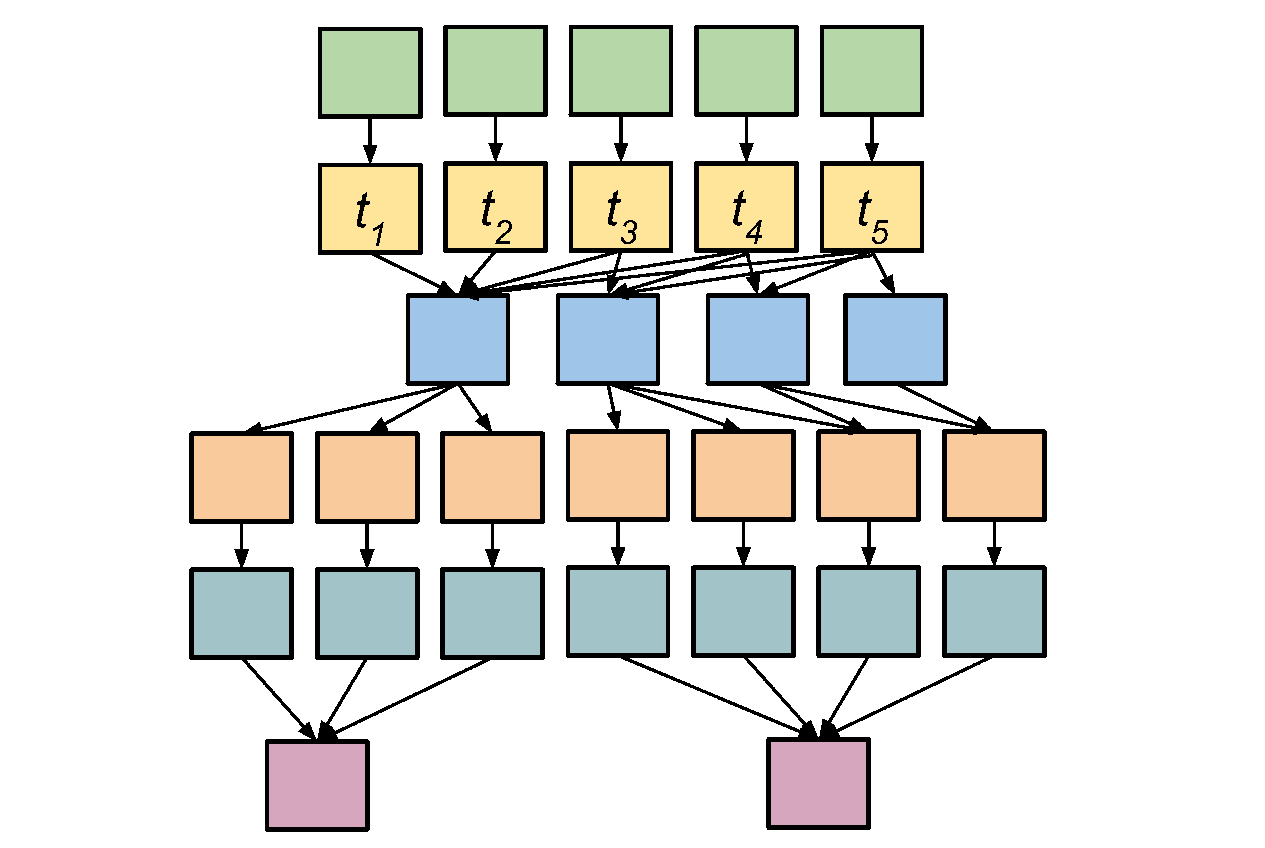
\includegraphics[width=0.85\linewidth]{figure11.eps}
	\captionof{figure}{A workflow example where HDB yields lower performance than HIFB. HDB does not capture the difference in the number of parents/child tasks, since the distances between tasks ($t_1$, $t_2$, $t_3$, $t_4$, and $t_5$) are the same.}
	\label{fig:imbalance_hifb_hdb}
\end{figure}

%In conclusion,  
Table~\ref{tab:2} summarizes the imbalance metrics and balancing methods introduced in this section. These balancing methods have different preference\rev{s when selecting }a candidate job to be merged. For instance, HIFB tends to group tasks that share similar importance to the workflow structure, while HDB tends to group tasks that reduce data transfers.

\begin{figure}[htb]
	\centering
	\small
	\begin{tabular}{l|l}
		\hline
		\textbf{Imbalance Metrics} & $abbr.$   \\
		\hline
		Horizontal Runtime Variance & \emph{HRV}   \\ 
%		%Pipeline Runtime Variance &{\em PRV}  \\ 
		Horizontal Impact Factor Variance & \emph{HIFV} \\ 
		Horizontal Distance Variance & \emph{HDV}  \\ 
		\hline
		\textbf{Balancing Methods} & $abbr.$  \\
		\hline
%		Horizontal Clustering & HC \\
		Horizontal Runtime Balancing & HRB   \\ 
%		Vertical Clustering & VC \\ 
		Horizontal Impact Factor Balancing & HIFB\\ 
		Horizontal Distance Balancing & HDB \\ 
		\hline
	\end{tabular}
	\captionof{table}{Summary of imbalance metrics and balancing methods.}
	\label{tab:2}
\end{figure}



\subsection{Combining vertical clustering methods}

In this subsection, we discuss how we combine the balanced clustering methods presented above with vertical clustering (VC).
%For one example workflow shown in Figure~\ref{fig:imbalance_vc}, we may simply merge tasks at the fourth level and tasks at the fifth level vertically. 
In pipelined workflows (single-parent-single-child tasks), vertical clustering always yields improvement over a baseline, non-clustered execution because merging reduces system overheads and data transfers within the pipeline. Horizontal clustering does not have the same guarantee since its performance depends on the comparison of system overheads and task durations. However, vertical clustering has \rev{a }limited performance improvement if the workflow does not have pipelines. Therefore, we are interested in the analysis of the performance impact of applying both vertical and horizontal clustering in the same workflow. We combine these methods in two ways: (\emph{i}) \emph{VC-prior}, and (\emph{ii}) \emph{VC-posterior}.


%\label{sec:vertical}
%\begin{figure}[htb]
%	\centering
%	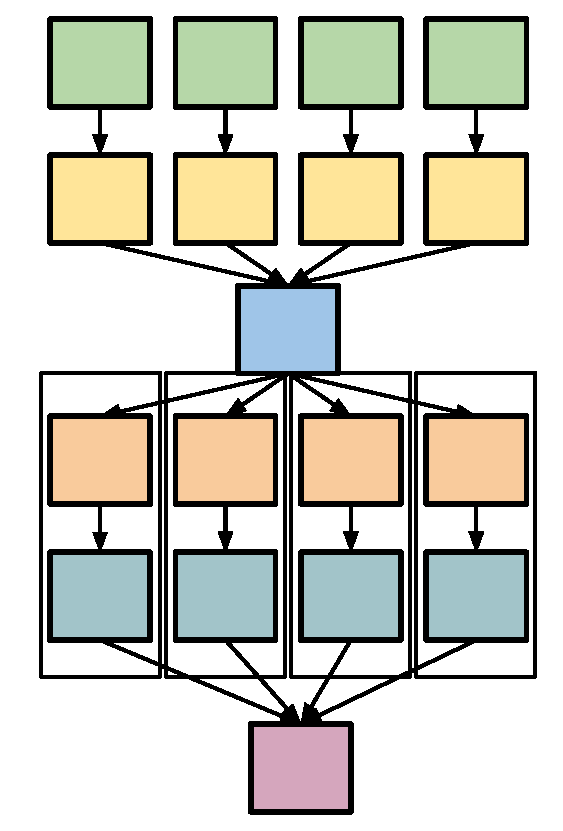
\includegraphics[width=0.35\linewidth]{figures/imbalance/vertical_clustering.eps}
%	\captionof{figure}{An example of Vertical Clustering.}
%	\label{fig:imbalance_vc}
%\end{figure}

\paragraph{\textbf{VC-prior}}
In this method, vertical clustering is performed first, and then the balancing methods (HRB, HIFB, HDB, or HC) are applied. Figure~\ref{fig:imbalance_vc_prior} shows an example where pipelined-tasks are merged first, and then the merged pipelines are horizontally clustered based on the runtime variance.

\begin{figure}[!htb]
	\centering
	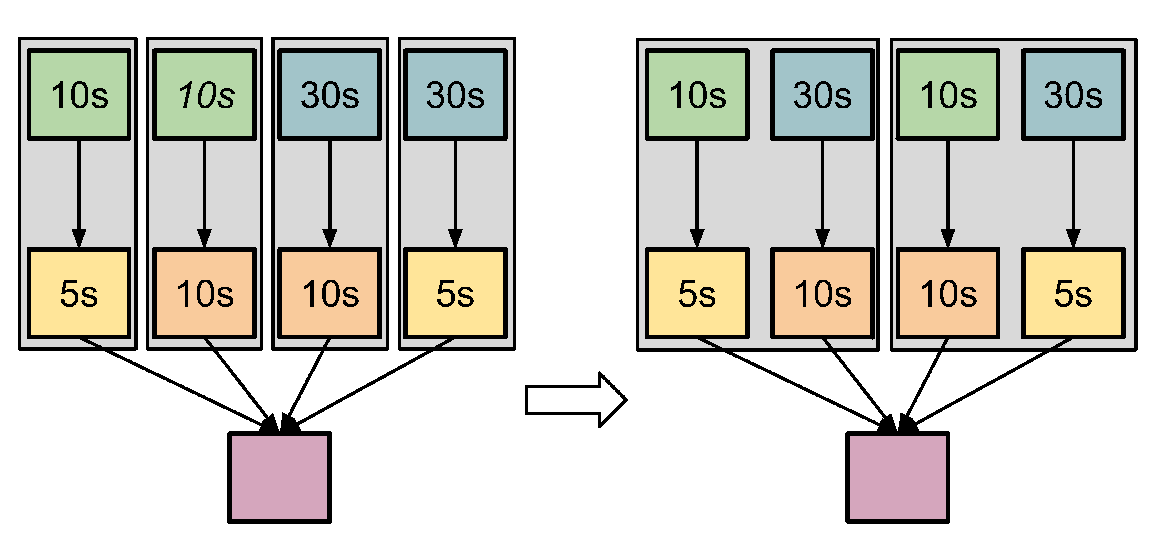
\includegraphics[width=0.85\linewidth]{figure12.eps}
	\captionof{figure}{\emph{VC-prior}: vertical clustering is performed first, and then the balancing methods.}
	\label{fig:imbalance_vc_prior}
\end{figure}

\paragraph{\textbf{VC-posterior}} 
%Here, vertical clustering is performed \emph{a posteriori}, i.e. balancing methods are first applied, and then VC. Figure~\ref{fig:imbalance_vc_posterior} shows an example where tasks are horizontally clustered first based on the runtime variance, and then merged vertically. In this example, vertical clustering targeted the data locality problem by merging tasks that would not generate interdependency once clustered. However, this approach causes a runtime imbalance problem.

\begin{figure}[!htb]
	\centering
	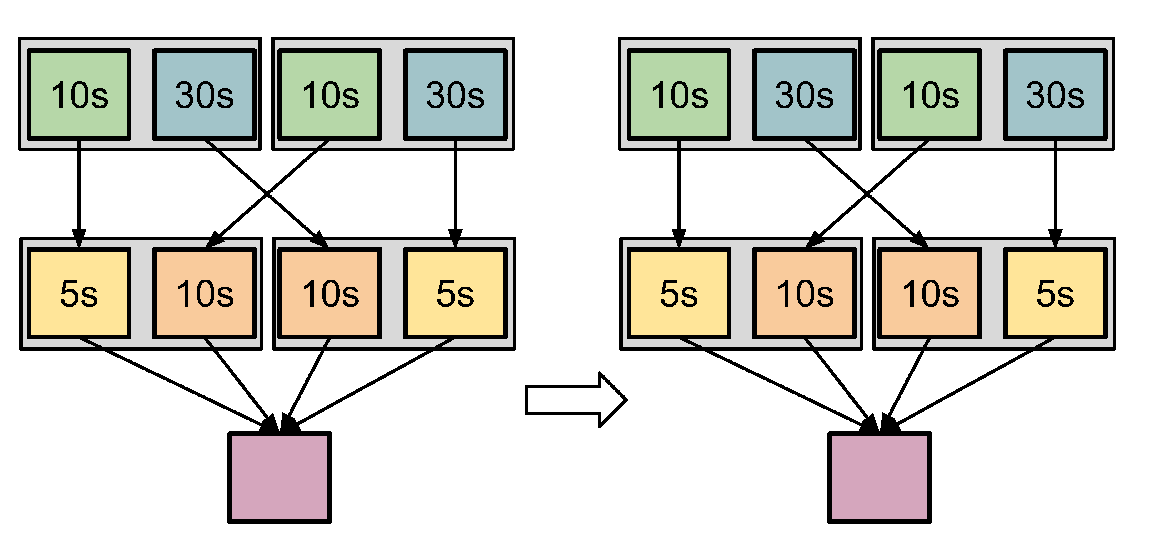
\includegraphics[width=0.85\linewidth]{figure13.eps}
	\captionof{figure}{\emph{VC-posterior}: horizontal clustering (balancing methods) is performed first, and then vertical clustering (but without changes).}
	\label{fig:imbalance_vc_posterior}
\end{figure}

Here, \rev{horizontal }balancing methods are first applied, and then vertical clustering \rev{is performed}. Figure~\ref{fig:imbalance_vc_posterior} shows an example where tasks are horizontally clustered first based on the runtime variance, and then merged vertically. However, since the original pipeline structures have been broken by horizontal clustering, VC does not perform any changes to the workflow. 


%means we perform horizontal clustering methods first and then vertical clustering. For the same workflow, assuming we merge tasks horizontally as shown in , we can see that we cannot perform vertical clustering to clustered jobs at the fourth level and the fifth level since the original pipeline structures have been destroyed by horizontal clustering. This phenomenon suggests us VC-posterior may work better compared to VC-prior, generally speaking. However, some opposite cases do exist. We will verify our hypothesis in Section~\ref{sec:results}. We will also compared the two combining approaches with \textbf{VC-only}, which means we perform vertical clustering only and \textbf{No-VC}, which means we just perform horizontal clustering methods without vertical clustering. 






